\documentclass[tikz,margin=10pt]{standalone}
\usepackage{tikz}
\begin{document}
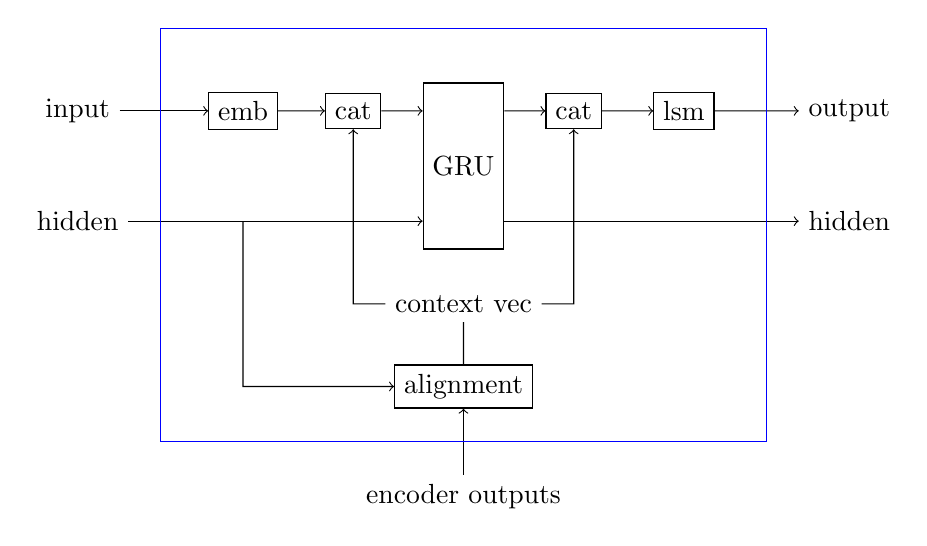
\begin{tikzpicture}[scale=.7]
	\node at (-7,2) (inp) {input};
	\node at (-7,0) (hid1) {hidden};
	\node at (7,2) (outp) {output};
	\node at (7,0) (hid2) {hidden};
	\node at (0,-1.5) (cnxt) {context vec};
	\node at (0,-5) (encout) {encoder outputs};

	\node at (-4,2) [rectangle, draw] (emb) {emb};
	\node at (-2,2) [rectangle, draw] (cat1) {cat};
	\node at (0,1) [rectangle, minimum height=6em, draw] (GRU) {GRU};
	\node at (2,2) [rectangle, draw] (cat2) {cat};
	\node at (4,2) [rectangle, draw] (lsm) {lsm};
	\node at (0,-3) [rectangle, draw] (align) {alignment};

	\draw [->]
	  (inp) edge (emb)
	  (emb) edge (cat1)
	  (cat1) edge (cat1-|GRU.west)
	  (GRU.east|-cat2) edge (cat2)
	  (cat2) edge (lsm)
	  (lsm) edge (outp)
	  (encout) edge (align)

	  (hid1) edge (hid1-|GRU.west)
	  (GRU.east|-hid2) -- (hid2)
	;

	\draw [->] (-4,0)--(-4,-3)--(align);
	\draw [->] (align)--(cnxt)--(-2,-1.5)--(cat1);
	\draw [->] (cnxt)--(2,-1.5)--(cat2);
	\draw [blue] (-5.5,-4) rectangle (5.5,3.5);

\end{tikzpicture}
\end{document}